%\documentclass[a3paper]{article}
%\usepackage[left=0mm,top=1cm,right=0mm,bottom=0mm]{geometry}
\documentclass[border=0]{standalone}
\usepackage{tikz}
\usepackage{xcolor}
\definecolor{pGreen}{HTML}{006633}
\definecolor{pRed}{HTML}{cc0033}

\begin{document}
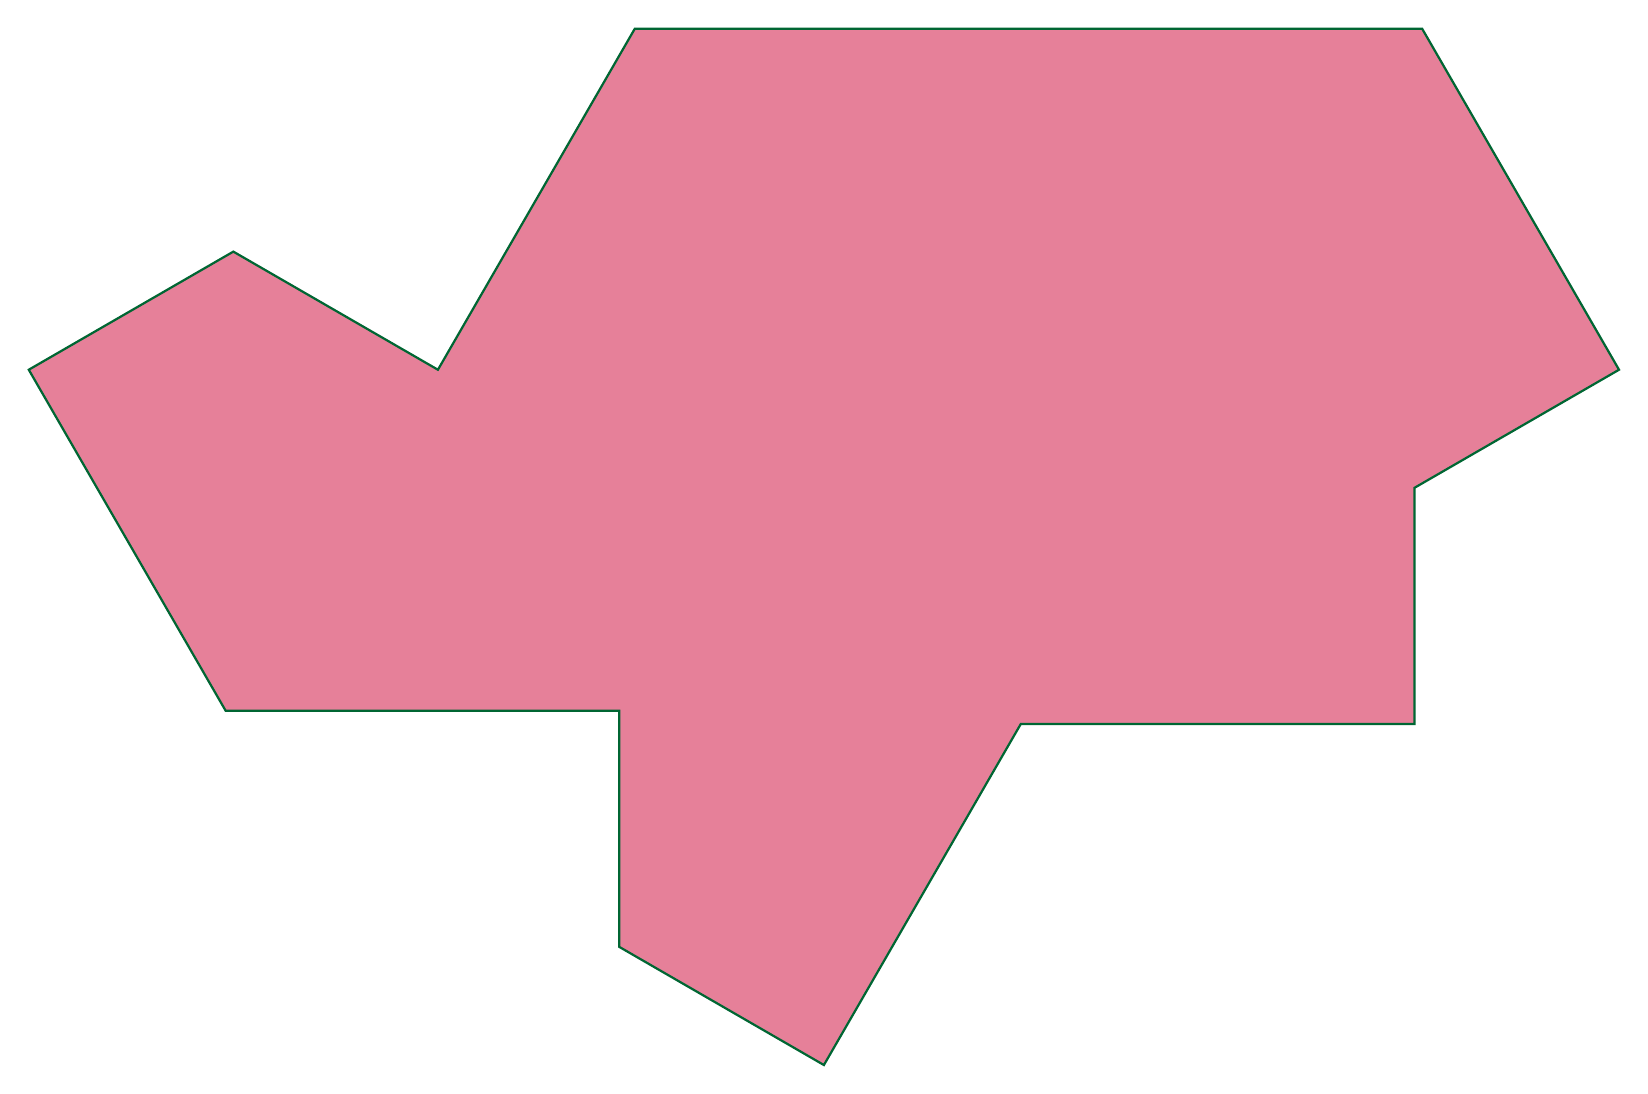
\begin{tikzpicture}
    \pgfmathsetmacro{\w}{1}	%scale
	\pgfmathsetmacro{\a}{5}
	\pgfmathsetmacro{\b}{3}
    \tikzset{
        monotile/.pic={
            \filldraw[draw=pGreen, fill=pRed!50, thick] (0,0) --++(-90:{\a*\w})--++(0:{\b*\w})--++(-60:{\b*\w})--++(30:{\a*\w})--++(90:{2*\a*\w})--++(150:{\w*\a})--++(60:{\w*\b})--++(120:{\w*\b})--++(-150:{\w*\a})--++(-90:{\w*\a})--++(180:{\w*\b})--++(-120:{\w*\b})--cycle;
        }
    };
	\draw(0,0) pic[rotate=90] {monotile};
\end{tikzpicture}
\end{document}
